\documentclass[prd,twocolumn,aps,psfig,nobibnotes,superscriptaddress,preprintnumbers,times]{revtex4}

\bibliographystyle{apsrev4-1} 
\setlength{\topmargin}{-14mm}
\usepackage{graphicx,bm,color,braket,amsmath}
\usepackage{hyperref}
\graphicspath{{./images/}{./fig/}{./png/}}
\def\red{\textcolor{red}}
\def\blue{\textcolor{blue}}
\usepackage{subcaption}
\usepackage{amssymb}
\usepackage{amsmath}
\usepackage{xfrac}
\usepackage{mathrsfs}
\usepackage{bm}
\usepackage{cancel}

\usepackage{xcolor}
%\usepackage[usenames, dvipsnames]{color}
%\usepackage{listings}
%\usepackage[square,numbers,sort&compress]{natbib}
%\usepackage{braket}
%\usepackage{nicefrac}
\usepackage{comment}

\usepackage{soul}
%%% \flag{...} marks text for MG to look at; delete the macro call to accept as-is.
\sethlcolor{yellow}
\newcommand{\flag}[1]{\hl{#1}}
\def \ul{\underline}
\def \vp{\varphi}

\def \ds{\displaystyle}
\def \pa{\partial}
\def \tcr{\textcolor{red}}
\def \tcb{\textcolor{blue}}


\newcommand{\neff}{N_{\rm eff}}
\newcommand{\dneff}{\Delta N_{\rm eff}}
\newcommand{\neffv}{N_{\rm eff}^{(\nu)}}
\newcommand{\nv}{N_{\nu}}
\newcommand{\dnv}{\Delta N_{\nu}}

\newcommand{\rad}{\rho_{\rm rad}}
\newcommand{\rel}{\rho_{\rm rel}}
\newcommand{\rb}{\rho_{\rm B}}
\newcommand{\extra}{\rho_{\rm extra}}

\newcommand{\ep}{e_{ij}^+}
\newcommand{\ec}{e_{ij}^\times}
\newcommand{\khat}{\hat{k}}
\newcommand{\kvec}{\mathbf{k}}
\newcommand{\hboost}{\tilde{h}}
\newcommand{\epp}{e_{ij}^{++}}
\newcommand{\ecc}{e_{ij}^{\times\times}}
\newcommand{\epc}{e_{ij}^{+\times}}
\newcommand{\ecp}{e_{ij}^{\times+}}
\newcommand{\eone}{\hat{e}^1}
\newcommand{\etwo}{\hat{e}^2}

%\newcommand{\Omgravitational wave}{\Omega_{\rm gravitational wave}}
%\newcommand{\Agravitational wave}{\mathcal{A}_{\rm gravitational wave}}
\newcommand{\n}{\hat{n}}
\newcommand{\vhat}{\hat{v}}
\newcommand{\p}{\hat{p}}
\newcommand{\z}{\hat{z}}
\newcommand{\x}{\hat{x}}
\newcommand{\y}{\hat{y}}
\newcommand{\that}{\hat{\theta}}
\newcommand{\ph}{\hat{\phi}}
\newcommand{\rhat}{\hat{r}}
\newcommand{\xb}{{\bf x}}

\newcommand{\bg}{\begin{equation}}
\newcommand{\bgg}{\begin{equation*}}
\newcommand{\en}{\end{equation}}
\newcommand{\enn}{\end{equation*}}

\newcommand{\infint}{ \int_{\infty}^{\infty}}

\newcommand{\mg}[1]{{\textcolor{red}{{[MG: #1]}}}}
\newcommand{\tb}[1]{{\textcolor{teal}{{[TB: #1]}}}}

\begin{document}
\title{Relic Gravitational Waves from Early-Universe Turbulence: Analytical Approach}
\date{\today}



\author{Murman Gurgenidze}
\email{mgurgeni@andrew.cmu.edu}
\affiliation{McWilliams Center for Cosmology and Department of Physics,
Carnegie Mellon University, Pittsburgh, PA 15213, USA}

\author{Tina Kahniashvili}
\email{tinatin@andrew.cmu.edu}
\affiliation{McWilliams Center for Cosmology and Department of Physics,
Carnegie Mellon University, Pittsburgh, PA 15213, USA}
\affiliation{School of Natural Sciences and Medicine, Ilia State University, 0194 Tbilisi, Georgia}
\affiliation{Abastumani Astrophysical Observatory, Tbilisi, GE-0179, Georgia}

\begin{abstract}

\end{abstract}

\maketitle

%\tableofcontents

Current cosmological observations, including  precise data from cosmic microwave background (CMB) anisotropies and large scale structure (LSS) surveys together with light element abundances, provide us with the universe picture from the moment of big bang nucleosynthesis (BBN) till today. However,  the earlier moments remain hidden. On the other hand, testing these moments is an invaluable possibility to get information about fundamental physics acting on extreme energies
\cite{Planck:2018vyg,Fields:2019pfx,Maggiore:1999vm,Dent:2024bhi,Roshan:2024qnv}.

The recent discovery of the stochastic gravitational wave background (SGWB) through pulsar timing arrays (PTAs) increased  interest in GW astronomy. Even though it is unlikely that the signal is from the early universe, such a possibility is not excluded. The violent processes in the early universe just shortly after inflation, such as preheating/reheating, cosmological phase transitions and follow up primordial turbulence, and/or magnetic fields, e.g. any anisotropic, traceless and traverse source can produce gravitational waves detectable by future detectors
\cite{NANOGrav:2023gor,RoperPol:2022iel,Khlebnikov:1997di,Caprini:2018mtu}.
The focus of this letter is to determine early-universe turbulence generated GWs spectral characteristics, potential detection prospects of these waves, and possibility to reconstruct (or limit) physical conditions much earlier than BBN
\cite{Kosowsky:2001xp,Gogoberidze:2007an,Caprini:2019egz}.

There are several conditions, under which primordial turbulence can develop (turbulence can develop if there is a mechanism injecting kinetic energy, whatever a source of sufficiently large-scale motions exists)
\cite{Caprini:2018mtu,Hindmarsh:2013xza,Brandenburg:1996fc,Joyce:1997uy}.
Turbulence is a complex nonlinear process controlled by multiple physical parameters, would it be produced in a laboratory or in the early universe. These parameters depend on each other, and the degeneracy between these parameters further complicates the appropriate modeling
\cite{Batchelor:1953,MoninYaglom:1975,Pope:2000}.
After inflation, when thermalized plasma has been formed, the fluid with ultra relativistic equation of state $ p =\rho/3$ with $p$ - pressure, and $\rho$ energy density) is characterized by two numbers, the hydrodynamic Reynolds number,
$\mathrm{Re} = {vL}/{\nu}$ and the magnetic Reynolds number, $\mathrm{Rm} = {vL}/{\eta}$
where $v$ is the characteristic velocity, $L$ is the characteristic length scale, $\nu$ is the kinematic viscosity, and $\eta=\sigma^{-1}$ is the magnetic diffusivity (in natural units), with $\sigma$ denoting the electrical conductivity. Their ratio defines the magnetic Prandtl number $\mathrm{Pm}={\mathrm{Rm}}/{\mathrm{Re}}={\nu}/{\eta}$.

During the radiation-dominated era, the primordial plasma was an excellent electrical conductor, resulting in an extremely small magnetic diffusivity. Consequently, the magnetic Reynolds number was many orders of magnitude larger than unity. The hydrodynamic Reynolds number was likewise very large, provided sufficient large-scale velocity perturbations were present, such as those generated during cosmological phase transitions or by chiral plasma instabilities. At the electroweak epoch ($T\sim100\,\mathrm{GeV}$), viscosity is dominated by weakly interacting particles (mainly neutrinos before decoupling), and typical estimates are
$\mathrm{Re}\sim10^{10}\text{--}10^{13},~~
\mathrm{Rm}\sim10^{16}\text{--}10^{20}$ yielding a magnetic Prandtl number $\mathrm{Pm}\sim10^{6}\text{--}10^{8}$. Thus, $\mathrm{Rm}\gg\mathrm{Re}\gg1 $.  
A similar hierarchy holds at the QCD phase transition ($T\sim150\,\mathrm{MeV}$), where estimates give  $\mathrm{Re}\sim10^{7}\text{--}10^{10}, ~~\mathrm{Rm}\gtrsim10^{17}$,
again implying $\mathrm{Pm}\gg1$
\cite{Son:1998my,Jedamzik:1996wp,Banerjee:2004df,Durrer:2013pga,Subramanian:2015lua}.

It should be highlighted that neither the Reynolds number nor the magnetic Reynolds number is a fundamental parameter. Both depend on the characteristic velocity and length scale of the flow. The values quoted above correspond to motions on the energy-containing (stirring) scale, typically assumed to be a fraction of the Hubble radius at the corresponding epoch. While the precise numerical values therefore depend on the plasma properties, it is safe to assume that both Reynolds numbers are overwhelmingly larger than unity \flag{throughout the radiation era. nonlinear advection dominates over viscous dissipation, leading magnetic fields remain effectively frozen into the plasma,}\tb{[the connective was lost here: the sentence breaks after ``radiation era.'' and ``leading'' has no verb. Reads as though it should be ``\ldots\ throughout the radiation era, so that nonlinear advection dominates over viscous dissipation, leaving magnetic fields effectively frozen into the plasma\ldots''} and ideal magnetohydrodynamic (MHD) turbulence laws apply, including inverse transfer and inverse cascade processes for helical fields.  Obviously,  direct numerical simulations (DNS) cannot reproduce the realistic physical parameters and instead rely on scaling laws to extrapolate from accessible Reynolds numbers
\cite{RoperPol:2019wvy,Kahniashvili:2020jgm,Auclair:2022jod,Schekochihin:2020aqu}.


\section{Methods}

\tb{Draft for MG to rewrite. Each subsection is either imported from the companion
(numbers already computed and validated there) or flagged NEW, meaning it still has to
be written from scratch. Kept deliberately terse.}

\subsection{The three inputs}

The GW spectrum from a turbulent source is fixed by three things: the equal-time spatial
spectrum of the fluid, the unequal-time correlator (UETC) of the anisotropic stress, and
the dissipation physics that terminates the cascade. They are not on an equal footing.
The strict $k\to0$ infrared slope follows from the spatial model alone by causality
\cite{Cai:2019cdl}; the ultraviolet asymptote from the temporal model alone
\cite{Zhou:1996,Rubinstein:2000}; the peak and the break from both. The observable band
is intermediate, so both matter.

\subsection{Dissipation: when it can be dropped, and why}

It is usually argued that the dissipation range is immaterial because the bulk of the GW
signal is produced faster than the turbulence decays \cite{Auclair:2022jod}. That is
correct but incomplete: it addresses the cutoff wavenumber, not the stress the
dissipation range carries. At $\mathrm{Pm}\gg1$ the field cascades past the viscous scale
$k_\nu$ to the resistive scale $k_\eta=k_\nu\sqrt{\mathrm{Pm}}$, and because the source
is $B_iB_j$ that range radiates. Feeding the Kulsrud--Anderson spectrum
\cite{Kulsrud:1992rk,Schekochihin:2003bg} through the kernel shows the contribution
appears only above $p\simeq2k_\nu/k_0$: the infrared is unchanged to two or three per
cent even at $\mathrm{Pm}=10^{8}$. The viscous contribution to the correlator is flat
below the inverse decorrelation time and adds no power of $k$. Dissipation may therefore
be dropped in the observable band --- as a conclusion, not an assumption.

\begin{figure*}[t]
  \centering
  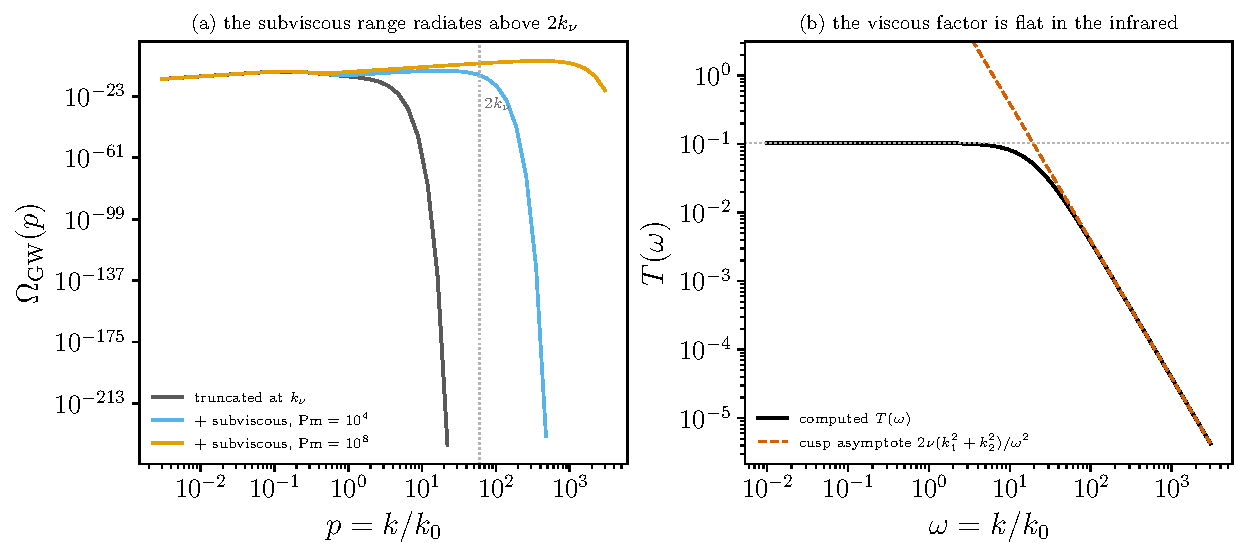
\includegraphics[width=0.86\textwidth]{subviscous_gw}
  \caption{The $\mathrm{Pm}\gg1$ dissipation range and the gravitational-wave band.
  (a)~Adding a subviscous magnetic range to a fixed large-scale field changes
  $\Omega_{\rm GW}$ only above $p\simeq2k_\nu/k_0$ (dotted line); the infrared is
  unchanged to two or three per cent even at $\mathrm{Pm}=10^{8}$, because two stress
  legs near $k_\nu$ can only radiate at $k\lesssim2k_\nu$. (b)~The two-leg viscous
  temporal factor, computed rather than extrapolated from its large-$\omega$ asymptote
  (dashed): it is flat below the inverse decorrelation time and so contributes no power
  of $k$ where the detectors look. The missing physics is real and lives in the far
  ultraviolet.}
  \label{fig:subviscous}
\end{figure*}

\subsection{Transport coefficients and their temperature dependence}

\tb{NEW --- not in the companion; references are in the bibliography and uncited.}
The kinematic viscosity is set by the dominant weakly-interacting species and the
resistivity by collisional processes, so $\nu$ and $\eta$ scale differently with $T$
\cite{Arnold:2000dr,Baym:1997gq}. Two regimes matter. While a species is coupled the
damping is diffusive, $\propto\nu k^{2}$; once it free-streams the damping becomes a drag
with a $k$-independent rate
\cite{Jedamzik:1996wp,Subramanian:1997gi,Banerjee:2004df}. Before neutrino decoupling
$\mathrm{Re}$ is large whatever the details, so the distinction does not bite. After
decoupling the free-streaming neutrinos raise the effective viscosity, so $\nu$ grows
between the QCD and electroweak epochs in both conformal and physical variables.
\tb{TODO: numbers --- $\nu(T)$, $\eta(T)$ and the resulting $\mathrm{Pm}(T)$ across the
two transitions. This is the one part of Methods that is genuinely new work.}

\subsection{Why Kraichnan sweeping does not transfer to the decaying case}

Two objections, of different weight. First, the decorrelation rate: random sweeping gives
$\tau_c\propto k^{-1}$ while the Kolmogorov turnover gives $k^{-2/3}$, and the GW problem
is posed in the Eulerian frame, where the former applies
\cite{Kraichnan:1964,Niksa:2018ofa}. Most treatments nevertheless adopt the turnover
time, including for magnetic sources. Second, and stronger: the shape of the correlator
at zero lag decides the ultraviolet, and it is measurable. Hydrodynamic simulations give
a Gaussian velocity UETC \cite{Auclair:2022jod}, hence no cusp. For the magnetic stress,
a parameter-free forward model of a published run reproduces the radiated energy for
cuspless correlators and overpredicts it by one to two orders of magnitude for cusped
ones. Power-law decorrelation of the BK2016 type \cite{Brandenburg:2016odr} is therefore
excluded for this class of source.

\begin{figure}[t]
  \centering
  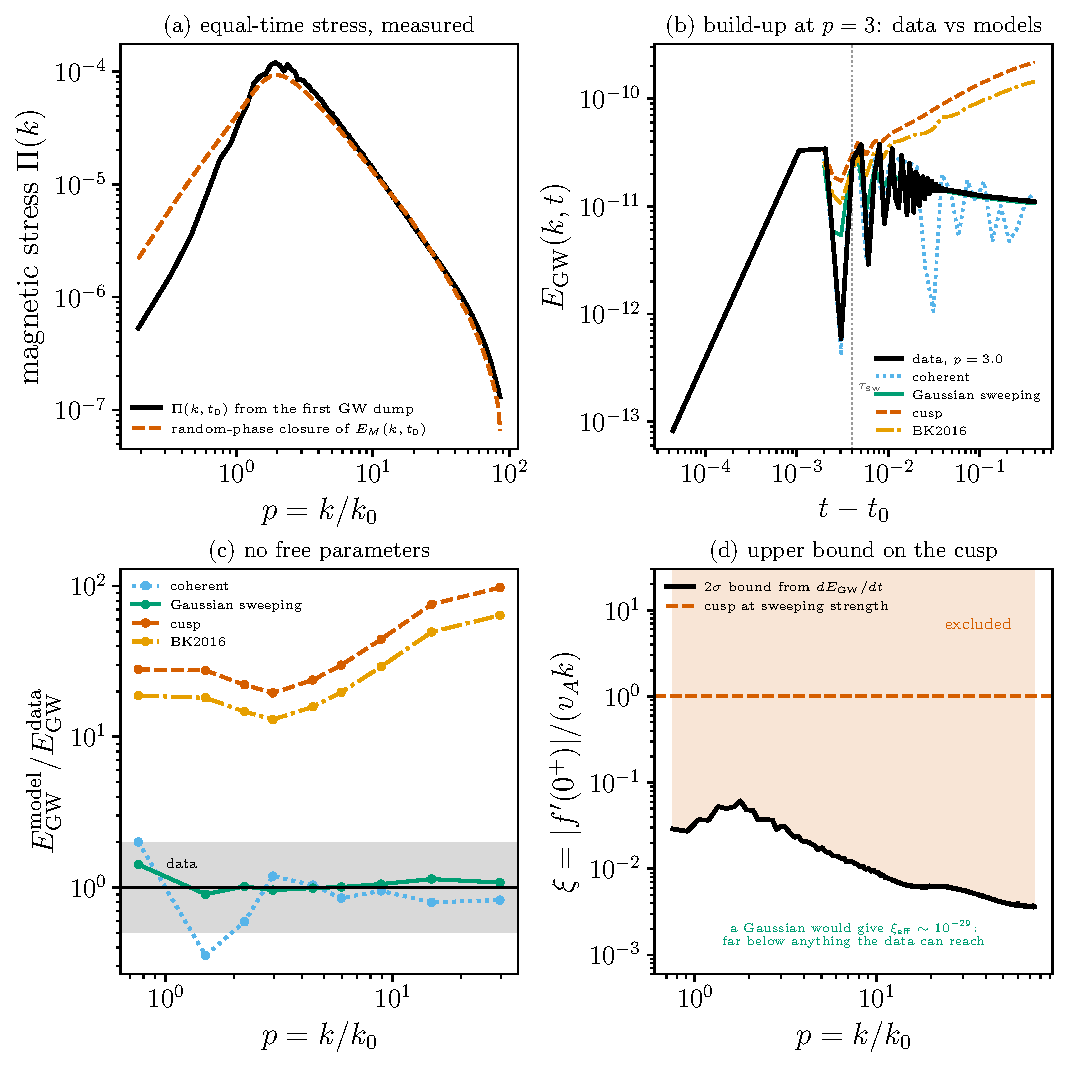
\includegraphics[width=\columnwidth]{magnetic_uetc}
  \caption{Constraining the magnetic stress correlator without two-time data. Because
  the simulation starts from rest, its gravitational-wave field is a running cosine
  transform of the stress correlator evaluated on the light cone, so the radiated energy
  at the end of the run is a prediction for each candidate correlator once the stress and
  the Alfv\'en speed are read off --- nothing is fitted. Cuspless correlators reproduce
  the measured energy; cusped ones overpredict it by one to two orders of magnitude.}
  \label{fig:magnetic-uetc}
\end{figure}

\subsection{Where the peak sits, and what moves it}

For a statistically stationary source decorrelating by sweeping, the peak is at
$p_{\rm peak}=\xi_\ast M$ with $\xi_\ast=1.488$ --- far below the source scale for
subsonic $M$. For a source of finite lifetime it sits at the source scale instead. The
mechanism is the emission \emph{window}, not the decorrelation: a source that starts and
stops carries a break at $2.33/W$, and that is what displaces the peak. Since the
magnetic correlator has no usable cusp, this is the operative case.

\begin{figure*}[t]
  \centering
  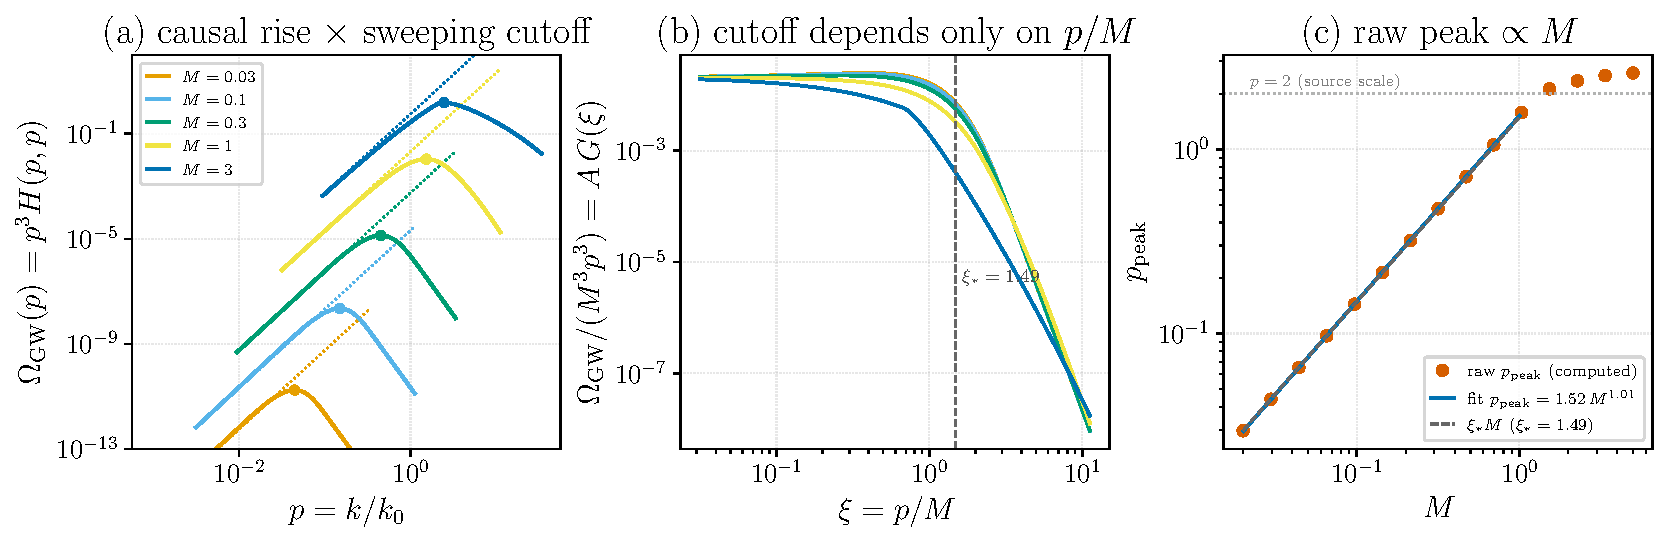
\includegraphics[width=0.94\textwidth]{stationary_peak_analysis}
  \caption{The peak of the stationary sweeping kernel. Spectra at different Mach number
  collapse onto a single curve in the sweeping variable $\xi=p/M$, so the peak is at a
  fixed $\xi_\ast=1.488$ and therefore at $p_{\rm peak}\simeq1.5\,M$ --- far below the
  source scale for subsonic $M$. A source of finite lifetime places it at the source
  scale instead; the displacement is caused by the emission window, not by the shape of
  the decorrelation.}
  \label{fig:peak}
\end{figure*}

\subsection{Initial conditions and the onset}

\tb{NEW --- partly open.} The spectrum is laid down while the source switches on, not by
sustained radiation from a developed cascade: in the run we analyse, the GW energy
saturates within a fraction of a sweeping time at every $k$. Two questions follow that we
cannot yet answer. Is a Kolmogorov spectrum present from the outset, or does the
transition itself radiate while the cascade establishes? And what is the transition time?
Both bear on how far the preceding result generalises, since that run starts from an
\emph{imposed} field rather than a physical transition.

\begin{figure}[t]
  \centering
  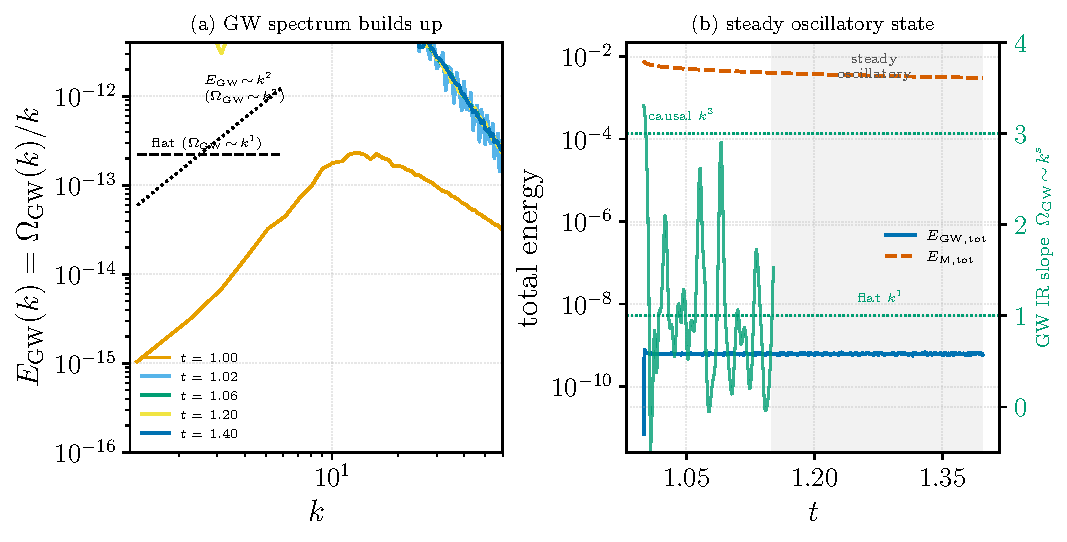
\includegraphics[width=\columnwidth]{roperpol_timeseries}
  \caption{The onset, resolved in time. The gravitational-wave spectrum is laid down
  while the source switches on rather than by sustained radiation from a developed
  cascade: the causal slope is a transient at switch-on and saturates within a fraction
  of a sweeping time at every wavenumber in the box. Whether a Kolmogorov spectrum is
  present from the outset, and how long the transition takes, remain open.}
  \label{fig:onset}
\end{figure}

\mg{Residual checklist. Covered above: fast-vs-slow dissipation; Kraichnan critique; peak
dynamics; plasma parameters (in the introduction); onset. Still to write: temperature
dependence of $\nu$ and $\eta$ with numbers; whether K41 holds from the start and the
transition time; conformal coordinates for the slow case.}

\bibliographystyle{apsrev4-1}
\bibliography{bib}

\end{document}
